\documentclass[conference]{IEEEtran}

% Note: 
% The layout of this tex file was generated by GenAI (chatgpt), based on a template design provided in an other course

% ------------------------------------------------------------
% PAGE LAYOUT
% ------------------------------------------------------------
\usepackage[paperwidth=210mm,paperheight=297mm,
            left=20mm, right=15mm, top=25mm, bottom=20mm,
            columnsep=5mm]{geometry}

% ------------------------------------------------------------
% FONTS & ENCODING
% ------------------------------------------------------------
\usepackage[T1]{fontenc}
\usepackage[utf8]{inputenc}
\usepackage{times}                % Times New Roman-like text
\usepackage{microtype}            % better justification

% ------------------------------------------------------------
% SECTION TITLES
% ------------------------------------------------------------
\usepackage{titlesec}
% Sections in SMALL CAPS, 12pt, centered
\titleformat*{\section}{\normalfont\scshape\centering\small}
\titleformat*{\subsection}{\normalfont\bfseries\small}

% ------------------------------------------------------------
% ABSTRACT & KEYWORDS
% ------------------------------------------------------------
\usepackage{abstract}
\renewcommand{\abstractnamefont}{\normalfont\bfseries\small}  % "Abstract"
\renewcommand{\abstracttextfont}{\normalfont\itshape\small}   % body
\setlength{\absleftindent}{0pt}
\setlength{\absrightindent}{0pt}

\newcommand{\keywords}[1]{%
  \vspace{1ex}\par\noindent%
  \textbf{Keywords—}\small #1%
}

% ------------------------------------------------------------
% CAPTIONS
% ------------------------------------------------------------
\usepackage[font=small,labelfont=bf,labelsep=period,justification=centering]{caption}

% ------------------------------------------------------------
% TEXT
% ------------------------------------------------------------
\usepackage[utf8]{inputenc}
\usepackage{enumitem}

% ------------------------------------------------------------
% GRAPHICS
% ------------------------------------------------------------
\usepackage{float}
\usepackage{graphicx}

% ------------------------------------------------------------
% HYPERREF (optional)
% ------------------------------------------------------------
\usepackage[hidelinks]{hyperref}
\usepackage[
  separate-uncertainty = true,
  multi-part-units = repeat
]{siunitx}

% ------------------------------------------------------------
% TITLE BLOCK
% ------------------------------------------------------------
\makeatletter
\renewcommand\maketitle{%
  \begin{center}
    \small\itshape
    Computer Architectures, memorymanagment and interfacing, Electronics-ICT,\quad October 2025,\quad Bruges, Belgium
  \end{center}
  \vspace{2ex}

  \begin{center}
    {\fontsize{22}{24}\selectfont\bfseries\@title\par}      % Title
    \vspace{1.5ex}
    {\fontsize{14}{16}\selectfont
       Joey De Smet\quad Sam Decorte\par
    }
    \vspace{1ex}
    {\fontsize{9}{11}\selectfont
      Faculty of Engineering Technology, KU Leuven - Bruges Campus\\
      Spoorwegstraat\,12, 8200 Bruges, Belgium\\
      \{joey.desmet, sam.decorte\}@student.kuleuven.be%
    }
    \vspace{2ex}
  \end{center}%
}
\makeatother

% ------------------------------------------------------------
% DOCUMENT
% ------------------------------------------------------------
\begin{document}

\twocolumn[{
  \date{October--2025}
  \title{Convolution Co-processor for ZYNQ7000 processing system}
  \maketitle
}]

% TODO
\begin{abstract}
% The abstract is a brief (50--80 words) synopsis of the paper. Use up to 5 keywords.
%Summary of the research and conclusion, Problem, method, results, conclusion....

\end{abstract}
\keywords{ Co-Processor, SIMD}


% ======================================================================================================================== %


\section{Introduction}

% TODO

% ======================================================================================================================== %


\section{Implementation}

% TODO

\begin{figure}[H]
\centering
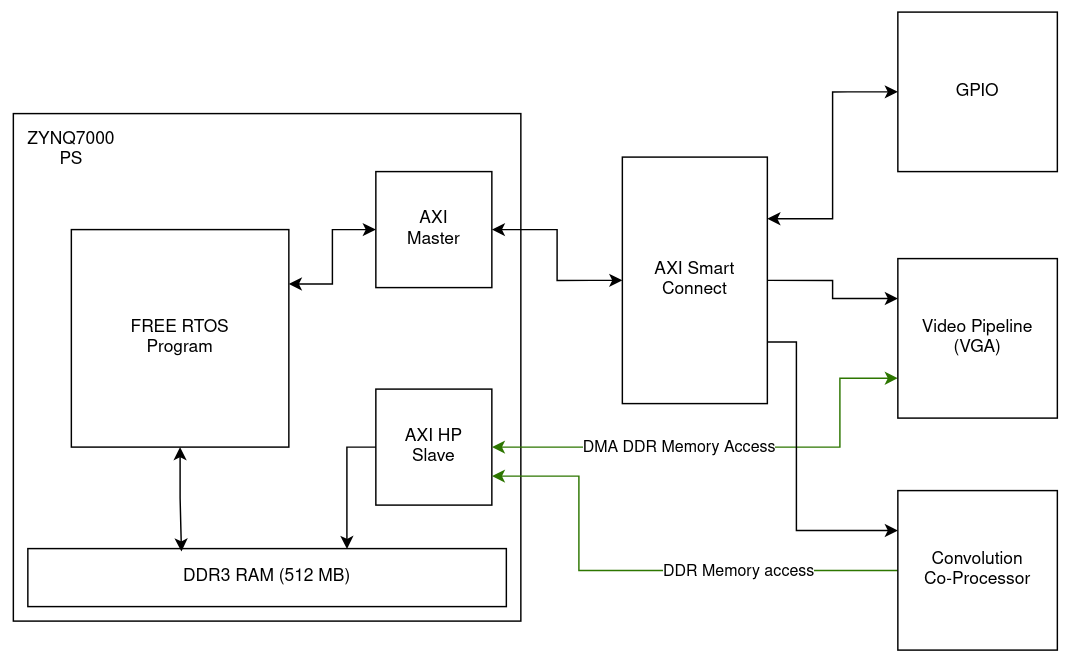
\includegraphics[width=0.45\textwidth]{images/Interconnect_architecture.png}
\caption{Overview interconnect architecture}\label{fig:firmware-system}
\end{figure}


% ======================================================================================================================== %


\section{Performance Analysis}

In this section, we evaluate the performance of the proposed convolution co-processor. Metrics include processing throughput, latency, resource utilization, and energy efficiency. Comparisons are made with a reference CPU-only implementation on the ZYNQ7000 processing system.

\subsection{Experimental Setup}
The experiments were performed on a Digilent ZedBoard development board with the following specifications:

\begin{itemize}[noitemsep]
  \item Processing System: Dual-core ARM Cortex-A9, 667 MHz
  \item FPGA: XC7Z020 (Artix-7), 53k LUTs, 106k FFs, 4.9 Mb BRAM
  \item Clock frequency of co-processor: \SI{100}{\MHz}
  \item Test images: resolution $640 \times 480$, 32-bit RGBA
  \item Convolution kernel: $3\times3$
\end{itemize}

\subsection{Latency and Throughput}

The latency $T_\text{latency}$ of the co-processor is measured as the time between issuing a convolution request and receiving the processed data:
\begin{equation}
T_\text{latency} = T_\text{transfer} + T_\text{compute} + T_\text{response}
\end{equation}

Throughput $R_\text{throughput}$ is calculated as:
\begin{equation}
R_\text{throughput} = \frac{\text{Number of pixels processed}}{T_\text{latency}}
\end{equation}

\begin{table}[H]
\centering
\caption{Latency and throughput for processing new versus in-memory images}
\begin{tabular}{c c c}
\hline
In memory & Latency [ms] & Throughput [MPix/s] \\
\hline
No & -- & -- \\
Yes & -- & -- \\
\hline
\end{tabular}
\label{tab:latency-throughput}
\end{table}

\subsection{Resource Utilization}

The FPGA resource usage of the convolution co-processor is summarized in Table~\ref{tab:resource-util}:

\begin{table}[H]
\centering
\caption{FPGA Resource Utilization}
\begin{tabular}{l c c}
\hline
Resource & Used & Available \\
\hline
LUTs & -- & -- \\
Flip-Flops & -- & -- \\
BRAM [Kb] & -- & -- \\
DSP Slices & -- & -- \\
\hline
\end{tabular}
\label{tab:resource-util}
\end{table}

\subsection{Comparison with CPU Implementation}

For reference, a CPU-only implementation, as a FreeRTOS task with highest priority, was run on the ARM Cortex-A9 core. Table~\ref{tab:cpu-vs-fpga} summarizes the speed-up achieved:

\begin{table}[H]
\centering
\caption{Speed-Up of FPGA Co-Processor vs CPU}
\begin{tabular}{c c}
\hline
CPU Latency [ms] & FPGA Speed-Up \\
\hline
-- & -- \\
\hline
\end{tabular}
\label{tab:cpu-vs-fpga}
\end{table}

% If possible and if we have time enough
\subsection{Energy Efficiency}

Energy consumption was measured for the convolution co-processor using onboard power monitoring or external measurement tools. The energy efficiency $\eta$ is defined as the number of pixels processed per joule of energy consumed:

\begin{equation}
\eta = \frac{\text{Number of pixels processed}}{E_\text{total}} \quad [\text{MPixels/J}]
\end{equation}

where $E_\text{total}$ is the total energy consumed during the convolution operation.

\begin{table}[H]
\centering
\caption{Energy efficiency of the co-processor for CPU and FPGA}
\begin{tabular}{c c c}
\hline
Platform & Energy [mJ] & Efficiency [MPix/J] \\
\hline
$FPGA$ & -- & -- \\
$CPU$ & -- & -- \\
\hline
\end{tabular}
\label{tab:energy-efficiency}
\end{table}


% ======================================================================================================================== %

\section{Conclusion}



% ======================================================================================================================== %

\section{Future work}

\begin{itemize}[noitemsep]
  \item Splitting the data into the different buffers to allow for more parallelism, is now managed by the processor. A hardware implementation could make it possible for data to be streamed in bigger burst which would decrease te delay for data transfer.
  \item Currently only $3\times3$ kernels are supported some minor changes could be done to expand this to a $n\times n $ kernel. 
\end{itemize}

% ======================================================================================================================== %

\section*{Acknowledgment}
The autors used generative AI tools to assist with language refinement, LaTeX table template generation and grammar correction during the preparation of this paper.

% ======================================================================================================================== %

\begin{thebibliography}{1}
\bibitem{ZedBoard User's Guide}
Digilent,
\textit{ZedBoard User's Guide},
2014.
Available: \url{https://files.digilent.com/resources/programmable-logic/zedboard/ZedBoard_HW_UG_v2_2.pdf}

\bibitem{ZedBoard User's Guide}
ARM,
\textit{AXI specification},
2025.
Available: \url{https://developer.arm.com/documentation/ihi0022/latest/}

\bibitem{Zynq 7000 SoC Technical Reference Manual}
AMD,
\textit{Zynq 7000 SoC Technical Reference Manual},
2023.
Available: \url{https://docs.amd.com/r/en-US/ug585-zynq-7000-SoC-TRM/Register-ICCIDR-Details}

\end{thebibliography}

\end{document}